\section{Oja's rule}

\mode<presentation>{
\begin{frame} 
    \begin{center} \huge
        \secname
    \end{center}
	%\begin{center}
	%Dealing with the diverging hebbian rule\\
	%through implicit normalization
	
	%\end{center}
	\svspace{5mm}
    \begin{center}
		\includegraphics[width=4cm]{img/meme_oja}
    \end{center}
\end{frame}
}

\begin{frame}{\secname}

Modify the update rule such that 
\begin{itemize}
\item it contains an 
\emph{implicit normalization} to prevent divergence and 
\item $\vec w$ still converges to the direction of the first PC.
\end{itemize}

\question{How?}

-By adding a \emph{decay term} to the update rule.

\begin{block}{Oja's rule:}
\begin{equation}
	\Delta {w}_j = \varepsilon~y_{ \big( \vec{x}^{(\alpha)}; \vec{w}
		\big) } \bigg\{ 
			\underbrace{ x_j^{(\alpha)} }_{
				\substack{	\text{Hebbian} \\
						\text{learning} }}
			- 
					\underbrace{
	y_{ \big( \vec{x}^{(\alpha)}; \vec{w} \big) } {w}_j
	}_{\text{decay term}}
			\bigg\}
\end{equation}
\end{block}

\end{frame}

\subsection{Alternative: Explicit normalization}

\mode<presentation>{   
\begin{frame}{Alternative to Oja's rule}

All Oja's rule does is:

\begin{itemize}
\item provide an
\emph{implicit normalization} to prevent divergence and 
still 
\item have $\vec w$ converge to the direction of the first PC.
\end{itemize}
	%\begin{center}
	%Dealing with the diverging hebbian rule\\
	%through implicit normalization
	%\pause
	%\end{center}
	\svspace{5mm}
    \begin{center}
		\includegraphics<2>[width=2cm]{img/smart_cookie}
		\includegraphics<3>[width=4cm]{img/meme_normalization}
    \end{center}
\end{frame}
}


\begin{frame}{\subsecname}

\begin{block}{Explicit normalization} 
i.e. keep $|\vec w| = 1$ after each step by normalizing it.

\begin{equation}
	\vec{w}(t+1) = 
    \frac{\vec w(t) + \Delta \vec w}{|\vec w(t) + \Delta \vec w|} 
    = \frac
    {\overbrace{\vec{w}(t) + {\only<3->{\color{blue}}\varepsilon y(\vec{x}^{(\alpha)}; \vec{w}(t))~\vec{x}^{(\alpha)}}}^{\text{Hebbian learning}}}
    {\underbrace{\left| \vec{w}(t) + \varepsilon y(\vec{x}^{(\alpha)}; \vec{w}(t))~\vec{x}^{(\alpha)} \right|}_{\text{Euclidean weights normalization}}}
    \label{eq:explicitnorm}
\end{equation}

\only<2>{
For the $j$-th component:\\
\begin{equation}
    w_j(t+1) = \frac
    {w_j(t) + \varepsilon y(\vec{x}^{(\alpha)}; \vec{w}(t))~x_j^{(\alpha)}}
    {\sqrt{ \sum_{k=1}^{N} \left( w_k(t) + \varepsilon y(\vec{x}^{(\alpha)}; \vec{w}(t))~{x_k}^{(\alpha)} \right)^2}}
\end{equation}

}



\end{block}

\notesonly{ 
Keep in mind that the above explicit normalization in \eqref{eq:explicitnorm}}
\only<3>{
uses the \textcolor{blue}{original hebbian update rule}
\notesonly{
$\color{blue}\Delta \vec w = \varepsilon y(\vec x^ {(\alpha)}; \vec w(t)) 
~\vec x^{(\alpha)}$} \underline{without} the decay term.}\notesonly{\\
If we were using the decay term, we wouldn't need an explicit normalization.
}

\only<4>{
\slidesonly{

    \begin{center}
		\includegraphics[width=3.5cm]{img/meme_decay}
    \end{center}
}
}
\end{frame}

\begin{frame}

\question{Does Oja's rule give different results than the explicit normalization?}\\

\notesonly{- No.\\}

\mode<presentation>{
\svspace{5mm}
\begin{center}
	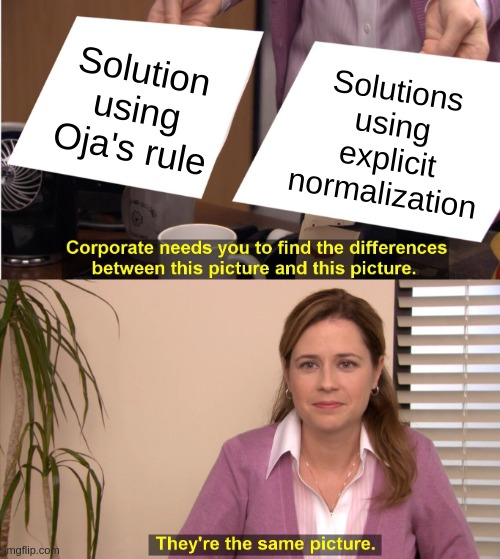
\includegraphics[width=3.5cm]{img/meme_ojaexplicit-same}
\end{center}
}

\pause

In the excercise sheet you will demonstrate that for small $\varepsilon$ the explicit normalization can be reduced to Oja's rule using a Taylor expansion around $\varepsilon = 0$ and neglecting terms of second or higher order in $\varepsilon$. 

\end{frame}
